\documentclass{article}
\usepackage[utf8]{inputenc}
\usepackage{tikz}
\usepackage{tkz-euclide}
\usepackage{bbm}
\usepackage{mathtools}
\usepackage{amssymb}
\usetikzlibrary{shapes.geometric}
\usetikzlibrary{calc,intersections,angles,quotes}
\title{Proof}
\author{Faris B. Mismar}
\date{September 2021}

\begin{document}

\maketitle

\section{Introduction}

Let an arbitrary star $\mathcal{S}$ have a length $\ell$ and $N$ points, with $N, \ell \in \mathbbm{Z}_{++}$.  The angle a graphics turtle would need to rotate is:
\begin{equation}
    \theta = \frac{360^\circ}{N} \times 2,
\end{equation}%
which has to repeat for $N$ times, after drawing a line segment of $\ell$ each time.

Let $\alpha$ be the measure of the circumferential angles formed by the vertices of the star $\mathcal{S}$ at the circumference of the inscribing circle.  It is easy to show that the radius of the circle $r$ splits $\triangle AXY$ into two identical triangles and therefore $\angle XAO = \alpha/2$.  Due to the same reason, the interior angle of the $N$-polygon formed by the star $\angle XOY = \frac{\theta}{4}$.

It should be easy to find out that $\alpha = 180^\circ - \theta$ since both angles fall on a straight line.

We inspect $\triangle AOB$ and $\triangle ADB$ knowing that $\angle ADB \coloneqq \alpha$.  Therefore, the central angle $\angle AOB$ sharing the same arc with the circumferential angle has the measure of $2\alpha$.

$\triangle AOB$ is an isosceles triangle with the base angle measure of $\gamma$.  Therefore, the measure of $\angle AOB$ is $\zeta \coloneqq 180^\circ - 2 \gamma$.  We can use the law of sines and write:

\begin{equation}
    \frac{r}{\sin \gamma}  = \frac{\overline{\rm AB}}{\sin \zeta},
\end{equation}
which makes it easy to write $r$ as
\begin{equation}
\begin{aligned}
r &= \overline{\rm AB} \frac{\sin \gamma}{\sin (180^\circ - 2\gamma)} \\
  &= \overline{\rm AB} \frac{\sin \gamma}{\sin 2\gamma} \\ 
  &= \overline{\rm AB} \frac{1}{\cos \gamma} \\ 
\end{aligned}
\end{equation}

We can write $\gamma$ in terms of the circumferential angle $\alpha$ by simply stating
\begin{equation}
    \gamma = \frac{1}{2} (180^\circ - 2\alpha) = 90^\circ - \alpha.
\end{equation}

Now we can write $r$ as follows
\begin{equation}
\label{eq:r_prelim}
r = \overline{\rm AB} \frac{1}{\sin \alpha}. \\ 
\end{equation}

We inspect $\triangle ABD$, which again is an isosceles triangle.  The base angles have the measure of $90^\circ - \alpha / 2$ each.  The law of sines enables us to write:

\begin{equation}
    \frac{\ell}{\sin(90^\circ - \alpha / 2)}  = \frac{\overline{\rm AB}}{\sin \alpha}.
\end{equation}

Here we can compute:

\begin{equation}
    \overline{\rm AB} =  \ell \frac{\sin \alpha}{\cos \alpha/2},
\end{equation}
where the use of the sine of the double angle trigonometry identity allows us to write $\overline{\rm AB} = 2\ell \sin \alpha/2$.  What is left now is finding substituting $\overline{\rm AB}$ in \eqref{eq:r_prelim} in terms of $\theta$ and $\ell$:

\begin{equation}
r = \frac{2 \ell \sin \alpha / 2}{\sin \alpha} = {\ell}\,{\cos \alpha / 2}
\end{equation}

\begin{equation}
\therefore r = \frac{\ell}{2} \frac{1}{\sin \theta /2} = \frac{\ell}{2}\, \csc \left ( \frac{360^\circ}{N} \right ) \qquad \blacksquare
\end{equation}

\begin{figure}[!t]
\centering
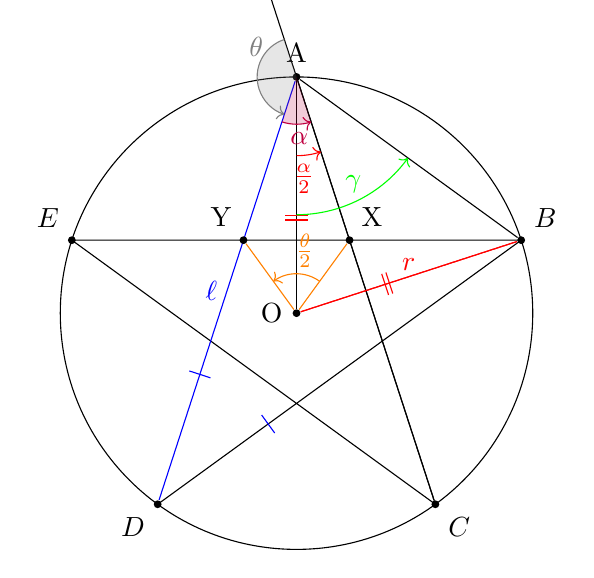
\begin{tikzpicture}[n/.style={circle, fill,inner sep=1pt}]
  \draw node [star, star point height=.5cm, minimum size=6cm,inner sep=0,outer sep=0] (s) {}
     circle (3) (s.outer point 1) node[n,label={90:A}] (A){} 
     foreach\x/\y in {4/C,2/E,5/B,3/D}{--(s.outer point \x) node[n,label={(-45+90*\x):$\y$}] (\y) {}}; %--cycle;

\draw [shorten >= -1.5cm] (C) -- (A);
\coordinate (Aprime) at ($(A)!1.5cm!180:(C)$); % Define a point that is on the same line between A and C.

\draw node(s.outer point 0) {} node [n,label={180:O}] (O) {};

\draw[-] (O) -- (A) node[] (AO) {};
\draw[-,color=red] (O) -- (B) node[] (BO) {};
\draw[-] (A) -- (B) node[] (AB) {};

\draw[-,color=red] (B) -- (O) node[midway, yshift=0.15cm] {$r$};
\draw[-,color=blue] (A) -- (D) node[midway, xshift=-0.2cm] {$\ell$};

\node[n,black,label={60:X}] (X) at (intersection of  A--C and B--E){};
\node[n,black,label={120:Y}] (Y) at (intersection of  A--D and B--E){};

\draw[-,color=orange] (O) -- (X);
\draw[-,color=orange] (O) -- (Y);

\tkzMarkSegment[color=red,pos=.4,mark=||](O,A) 
\tkzMarkSegment[color=red,pos=.4,mark=||](O,B) 
\tkzMarkSegment[color=blue,pos=.3,mark=|](D,A) 
\tkzMarkSegment[color=blue,pos=.3,mark=|](D,B) 

\pic["$\frac{\alpha}{2}$" shift={(0pt,-20pt)},draw,color=red,->,angle radius=1cm] {angle = O--A--X};
\pic["$\gamma$" shift={(7pt,-12pt)},draw,color=green,->,angle radius=1.75cm] {angle = O--A--B};
\pic["$\theta$" shift={(-6pt,11pt)},draw,color=gray,->,fill=gray,fill opacity=0.2,text opacity=1,angle radius=.5cm] {angle = Aprime--A--Y};
\pic["$\frac{\theta}{2}$" shift={(3pt,14pt)},draw,color=orange,->,angle radius=.5cm] {angle = X--O--Y};
\pic["$\alpha$" shift={(1pt,-12pt)},draw,color=purple,->,fill=purple,fill opacity=0.2,text opacity=1,angle radius=.6cm] {angle = Y--A--X};

\end{tikzpicture}
\caption{Solving the triangles}
\end{figure}

\end{document}
